\chapter*{Introduction Générale}
\addcontentsline{toc}{chapter}{Introduction Générale}
Au cours des dernières décennies, nous avons assisté à une nouvelle tendance dans l'histoire de l'informatique : les chercheurs déplacent progressivement leur analyse de l'étude de l'individu vers celle du collectif. Nous pouvons percevoir ce changement dans de nombreux domaines. En combinant des données provenant de sources multiples, les chercheurs ont commencé à observer et à analyser le comportement collectif des foules [a.5], les changements physiques de notre environnement, les interactions sociales et monétaires des populations, la propagation des maladies et la consommation d'énergie dans les villes, entre autres.\\

Chacun de ces domaines présente des caractéristiques uniques. Pourtant, dans de nombreuses applications, notamment la détection, [b.3] la finance, l'épidémiologie et la biologie, on trouve une approche sous-jacente commune : la modélisation des dépendances d'entités interconnectées sous forme de graphes.\\

Pour tirer parti de cette nouvelle façon de représenter les données, de nombreux outils et techniques ont vu le jour. Les bases de données de graphes comme Neo4j, sont optimisées pour des requêtes avec lesquelles la base de données relationnelle peut facilement souffrir, ces requêtes contiennent généralement beaucoup de jointures, et même si les professionnels des bases de données relationnelles ont essayé pendant des décennies d'optimiser cela, le nombre de résultats intermédiaires peut croître exponentiellement en taille, ce qui peut parfois même remplir toute la mémoire disponible sur le disque.\\

Généralement, ces outils proposent leur propre langage de requête SQL, même si ces langages ont récemment convergé vers une syntaxe similaire, et donc une requête de sur un graphe, habituellement ressemblera à cela dans beaucoup de ces systèmes :\\
\begin{figure}[H]  
 \centering
    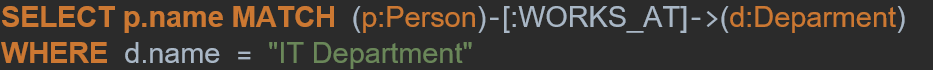
\includegraphics[width=1\textwidth]{exmp_pgql.PNG}
\end{figure}
Si nous supposons qu'il s'agit d'un site de commerce électronique, cette requête sélectionnera le nom de toutes les personnes travaillant dans le département informatique.\\
La même requête en SQL deviendra moins intuitive et ressemblera à ceci :
\begin{figure}[H]  
 \centering
    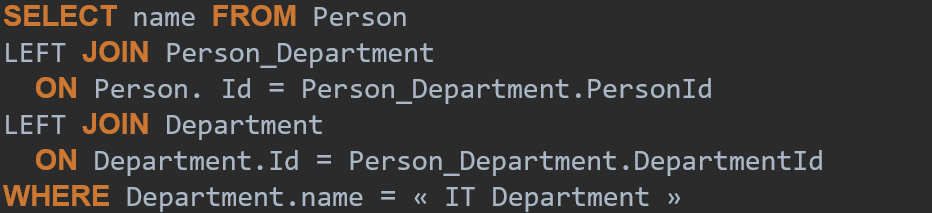
\includegraphics[width=1\textwidth]{exmp_sql.PNG}
\end{figure}

Le traitement de graphes gigantesques, des graphes pouvant atteindre des dizaines de téraoctets, présente ses propres défis. La recherche d’une faible latence nécessitera le chargement du graphe en mémoire pour le traiter, car la vitesse du disque est encore aujourd’hui très lente par rapport à la RAM. Peu de machines peuvent avoir assez de mémoire pour ce genre de charge de travail, et même si une machine avait autant de mémoire, que se passera-t-il si la taille augmente très rapidement, que la mise à l’échelle du nœud du calcule sera insuffisante ? Le système ne pourra pas contenir toutes ces données, et c’est là que PGX.D [a.2], [a.3] vient à la rescousse, puisque ce système est un système distribué, la mise à l’échelle par l’ajout d’autres nœuds serait naturelle et peut être moins coûteuse puisque vous pouvez n’utiliser que les machines que vous jugez nécessaires.\\
Dans ce rapport, je présenterai ma contribution au projet PGX.D ou je me concentrerai sur les points suivants :\\
\begin{itemize}[label=\textbullet]
\item Présentation de l’organisme d’accueil, et le projet PGX.
\item Présenter et expliquer des notions fondamentales pour comprendre ce système.
\item L’extension du support de filtrage, en ajoutant la possibilité de créer un sous-graph à partir d’une collection de sommets/bords ainsi que l’opération inverse.
\item Ajout du support aux propriétés NULL dans les « frames ».
\item Benchmarking avec TPC-H.
\end{itemize}

Des annexes seront proposées en fin du rapport pour développer quelques aspects clés qui n’ont pas été approfondis dans les différentes parties.